\PassOptionsToPackage{table}{xcolor}
\documentclass[manuscript,nonacm]{acmart}
\AtBeginDocument{%
  \providecommand\BibTeX{{%
    Bib\TeX}}}

\usepackage{amsmath}
\let\Bbbk\relax
\usepackage{amssymb}
\let\Bbbk\relax
\usepackage{pifont}
\usepackage{wasysym}
\usepackage{marvosym}
\usepackage{threeparttable}
\usepackage{textgreek}
\usepackage{paralist}
\usepackage{filecontents}
\usepackage{booktabs}
\usepackage{multirow}
\usepackage{tikz,siunitx}
\usetikzlibrary{shapes.geometric,shapes.symbols}
\usepackage{threeparttable}
\usepackage{enumerate}
\usepackage{comment}

% Commands for Surveyed Works Table
\newcommand{\cmark}{\ding{51}}%
\newcommand{\xmark}{\ding{55}}%
\newcommand{\markA}{\ding{66}}%
\newcommand{\markB}{\ding{71}}%
\newcommand{\markC}{\ding{75}}%
\newcommand{\markD}{\ding{168}}%
\newcommand{\markE}{\ding{169}}%
\newcommand{\markF}{\ding{170}}%
\newcommand{\markG}{\ding{171}}%
\newcommand{\markH}{\ding{92}}%
\newcommand{\markI}{\ding{214}}%
\newcommand{\markJ}{\ding{166}}%
\newcommand{\markX}{\Sagittarius} % heh
\newcommand{\markY}{\Virgo}
\newcommand{\markZ}{\Moon}
\newcommand{\markEtc}{\textbf{?}}
\def\rot{\rotatebox}
\newcommand*\circled[1]{\tikz[baseline=-3pt]{
            \node (X) [shape=circle,scale=0.5,fill=black,text=white,font=\bfseries, text centered, draw,inner sep=0pt] {\strut #1};}}
            
\newcommand{\wc}[1]{\textit{\textcolor{magenta}{#1}}} % Word-Choice macro
\newcommand{\maxnote}[1]{\textit{\textcolor{violet}{#1 --Max}}}
\newcolumntype{P}[1]{>{\centering\arraybackslash}p{#1}}

\begin{document}

\title{PLACEHOLDER}
\author{Max Gao}
% \authornote{Both authors contributed equally to this research.}
\affiliation{%
  \institution{CAIDA/UC San Diego}
  \city{San Diego}
  \state{CA}
  \country{USA}
}
\email{magao@ucsd.edu}

\begin{abstract}
For decades, analysis of network telescope traffic has consistently provided insights into Internet-wide phenomena, \textit{e.g.,} malicious scanning, backscatter from denial-of-service (DoS) attacks, and Internet outages, that impact the security and availability of the Internet.
To better operationalize darknets for their monitoring capabilities, researchers have proposed numerous methodologies that each aim to automate the detection of such events by employing a variety of techniques and leveraging different features of darknet traffic.
Yet despite an abundance of available methodologies, less attention has been directed towards comprehensive assessment of their comparative capabilities due to the availability of labeled datasets, replicability of methodologies, and a unified approach to method validation.
In this report, we survey existing works that propose and evaluate detection such methodologies, \dots

% Analysis of network telescope, or darknet, traffic has provided substantial visibility into the security and availability of the Internet for decades.
% To operationalize darknet monitoring capabilities, researchers have proposed numerous frameworks that automate the detection of Internet-wide events.
% Despite an abundance of available frameworks, less attention has been directed towards systematic comparison of their capabilities. 
% As a result, \dots
% In this report, we survey existing work that proposes and evaluates such frameworks on real-world darknet traffic.
% We review tasks that motivate the techniques each framework employs as well as experimental details of their evaluation; and finally, discuss future \dots
% To more effectively operationalize network telescopes for monitoring the security and availability of the Internet, researchers have proposed a diverse body of frameworks which codify empirical post-hoc analysis techniques.
% Yet, \dots
\end{abstract}

\maketitle

\section{Introduction}

Network telescopes, or darknets, have been instrumental to both researchers and practitioners for their ability to observe Internet-wide phenomena in the unsolicited traffic they receive. 
Over the past two decades, research efforts have shifted from characterizing darknet phenomena and their observable signals towards translating such empirical insights into operationalizable methodologies for monitoring the Internet's security and availability in near real-time.
% This has resulted in a number of methodologies that each leverage different approaches to achieve a common goal of broadly automating darknet event detection. 
% \maxnote{see other papers for enumerating on specific details in intro} As security risks mount along growing volumes of darknet traffic, such methodologies represents a crucial and necessary transition from conventional post-hoc manual traffic analysis workflows. 
% However, the utility of these methodologies depend critically on their accuracy and validity which remain elusive to evaluate due to several challenges that we identify through our survey. 
These efforts have resulted in a variety of methodologies that share the common goal of broadly automating event detection while differing widely in the algorithmic techniques they employ (e.g., statistical forecasting, matrix decompositions, and graph-based models), 
the traffic features they exploit (e.g., packet counts, port sequences, temporal bursts), 
and their operational definition of what constitutes an event (ranging from short-lived scans to sustained probing campaigns).
As security risks mount along growing volumes of darknet traffic, such methodologies represent a crucial and necessary transition from post-hoc manual traffic analysis towards a more \maxnote{dots} means of detection.
However, the utility of these frameworks depend critically on their accuracy and validity, which remain elusive to evaluate due challenges posed by \dots.

% However, as we identify in our suvey, methodologies differ widely in several ways: the algorithmic techniques they employ (e.g., statistical forecasting, matrix decompositions, and graph-based models), the traffic features they exploit (e.g., packet counts, port sequences, temporal bursts), 
% and their operational definition of what constitutes an event (ranging from short-lived scans to sustained probing campaigns).

% Network telescopes, or darknets, have been instrumental to both researchers and practitioners due to their capacity to observe Internet-wide phenomena in the unsolicited traffic they receive. 
% The visibility afforded by these observatories have enabled significant progress in the areas of cybersecurity and censorship, evident in a rich body of work that centers around the study of malicious scanning, denial-of-service attacks, and Internet outages. 
% The visibility afforded by these observatories have enabled significant progress in the areas of cybersecurity and censorship, evident in a rich body of work centered around 
% malicious scanning, denial-of-service events, and Internet outages. 

% Over the past two decades, research efforts have shifted from characterizing darknet phenomena and their observable signals towards translating such empirical insights into operationalizable frameworks for monitoring the Internet's security and availability in near real-time.  
% This has led to the development of a number of frameworks that each share the common goal of automating the detection of events in darknet traffic while taking notably different approaches to doing so\maxnote{feedback: elaborate on the specifics here.}.
% As security risks mount along with growing volumes of darknet traffic, such frameworks represent a crucial and necessary transition from conventional post-hoc manual traffic analysis workflows.
% However, the utility of these frameworks, particularly those more recent that leverage machine learning techniques, depend critically on their accuracy and validity which remain elusive to evaluate due to challenges posed by the diversity of framework detection objectives and approaches.

% As a result, a number of frameworks that each share a common goal of automating event detection within darknet traffic have been proposed.
% This has resulted in a number of proposed frameworks that share a common goal of automating the detection of events within darknet traffic.
% \begin{enumerate}
%   \item Overview of topic - 2 sentences.
%   \item 
%   \item Summary of contributions - 3 sentences.
% \end{enumerate}

% Network telescopes, or darknets, have been instrumental to both researchers and practitioners due to their capacity to observe Internet-wide phenomena in the unsolicited traffic they receive.
% Over the past two decades, research efforts have shifted from characterizing such phenomena and their observable signals towards translating these empirical insights into operationalizable frameworks for monitoring the Internet's security and availability in near real-time.

% Network telescopes, or darknets, have been instrumental to both researchers and practitioners due to their capacity to observe Internet-wide phenomena in the unsolicited traffic they receive.
% Over the past two decades, research efforts have shifted from characterizing such phenomena and their observable signals towards translating empirical insights into operationalizable frameworks for monitoring the Internet's security and availability in near real-time.
% As a result, a large variety of frameworks have been proposed. 
% Each share the same general goal of automating event detection.
% They vary widely in their choice of techniques and selection of darknet traffic features as they are designed with different event definitions in mind.
% \textit{discuss why it's difficult to speculate on their performance without further empirical evaluation.}

% Despite the variety of available frameworks for darknet traffic analysis, selecting the most suitable framework off-the-shelf for a given darknet is challenging.
% While the variety of frameworks is frank

% Traffic Growth
% Complexity Growth - new 

In this report, we survey an extensive body of literature to construct a taxonomy of darknet event detection methodologies followed by a separate taxonomy that details their assessments in empirical evaluations. 
We begin with an overview of prior work that characterizes network telescope traffic and chronicles its major changes in Section~\ref{sec:bg}.
We then describe our taxonomy of methodologies in Section~\ref{sec:frameworks}, comparing\dots\maxnote{brief summary}, followed by a review of their evaluation in Section~\ref{sec:evaluations}.
Finally, using our survey's findings, we conclude with a discussion of challenges in this area as well as directions for future work in Section~\ref{sec:fw}.

% We begin this report with an overview of network telescopes, the traffic they collect, and the types of Internet-wide events inferrable through analysis of such traffic.
% We then survey various frameworks that have been proposed to automate event detection and construct a taxonomy that compares their 1) analysis goals and designs; and 2) performance as informed by empirical evaluations on real-world darknet traffic.
% Using this taxonomy, we identify challenges and opportunities for future research where efforts may yield improvements over the current state-of-art.

\label{sec:bg}
\section{Background}
In this section, we provide a brief overview of network telescopes and highlight their role in Internet measurement research.
We first discuss technical details of their function as sensors that provide visibility into Internet-wide activities. 
We then characterize the nature of their received traffic and summarize findings from major studies that have examined its composition and sources.
Finally, we highlight investigations of notable Internet events enabled by analyzing traffic observed by telescopes.

\label{sec:bg:nt}
\subsection{Network Telescopes}

% Brief overview of darknets and their traffic (IBR)
Network telescopes, or darknets, consist of IPv4 address space that receive, but do not respond to, unsolicited Internet traffic via routes announced through the Border Gateway Protocol (BGP).
For decades, researchers have studied this unidirectional traffic to understand its mixtures and origins, attributing its causes to Internet-wide activity ranging from 
malicious scanning~\cite{@@}, residual backscatter from DoS attacks~\cite{@@}, Internet outages~\cite{2011dainotti,2013benson,2015benson,2012dainotti,2021padmanabhan}, and non-trivial network misconfigurations~\cite{@@}.

\begin{enumerate}
    \item three types of Internet-wide activity (summarize findings from each of the past major works, characterization of IBR and its changes, major events studied)
\end{enumerate}

Studies of darknet traffic in 2003 by Yegneswaran et al.~\cite{2004yegneswaran} quantified the volume of traffic and distributions of senders responsible for originating malicious scans 
and estimated that 25 billion Internet-wide scans originate per day.
Pang et al.~\cite{2004pang}\dots
Casado et al.~\cite{2005casado}

% Characterization citations
~\cite{2004yegneswaran,2004pang}

% Outage
~\cite{2011dainotti,2013benson,2015benson,2012dainotti}~\cite{2021padmanabhan}

% Discuss IBR, how it's been analyzed, practical use-cases for security / outage detection

\label{sec:frameworks}
\section{Methodologies for Darknet Event Detection}
\section{Methodologies for Darknet Event Detection}

In this section, we provide a broad survey of existing methodologies that have been proposed for detecting various kinds of darknet activities.
We review the defining components that characterize each method and organize a taxonomy (shown in Table~\ref{@@} and visualized in Figure~\ref{@@}) which illustrates \maxnote{takeaway}.

% In this section, we broadly survey existing methodologies that have been proposed for detecting various types of darknet activities.
In this section, we provide a broad survey of existing methodologies that have been proposed for detecting darknet activities and 
organize prior works into a taxonomy that identifies the need for a systematic evaluation approach to account for the diversity of methods.
We structure our survey by categorizing detection methodologies primarily based on the type of darknet activity they aim to detect. 
Within these categories, we review and emphasize two important aspects of each methodology: 
1) the class(es) of general \textit{techniques} they employ for detection; and 
2) their definition(s) of an \textit{event} belonging under their broader type of targeted activity.
We briefly discuss these aspects before discussing the methodologies that comprise our taxonomy as shown in Figure~\ref{fig:taxonomy}.

Our survey structure consists of a top-level categorization of detection methodologies based on the broad class of (i) darknet activity they aim to detect.
Under these categories, we group similar methods by the (ii) general classes of techniques they employ to achieve their (iii) detection objectives.
Using these groupings, we summarize the intuition behind each method and elaborate on finer-grained details pertaining to their specific (iv) algorithms and (v) traffic features.
Here, we briefly discuss components of the methods we survey.

% We structure our survey by categorizing detection methodologies primarily based on the type of darknet activity they aim to detect. 
% Within these categories, we review and emphasize two important aspects of each methodology: 
% 1) the class(es) of general \textit{techniques} they employ for detection; and 
% 2) their definition(s) of an \textit{event} belonging under their broader type of targeted activity.
% We briefly discuss these aspects before discussing the methodologies that comprise our taxonomy as shown in Figure~\ref{fig:taxonomy}.


\vspace{0.25em}
\noindent{\textbf{Activity Type(s)}} correspond to existing categories of observed activities in darknet traffic as described in Section~\ref{sec:bg:nt}. 
For each study, we identify these type(s) based on explicitly stated goals of each methodology and empirical results from their evaluation. 
Some methods such as~\ref{@@} are capable of detecting multiple types of activities depending on whether their input traffic is filtered.

\vspace{0.25em}
\noindent{\textbf{Event Definitions}} refers to attributes represented in the outputs of a given framework.
These attributes derive from packet header fields and implicitly define an instance of a broader type of event.
For example, a framework may define a scanning event using a source-based schema that consists of a timestamp, source IP address, an assigned cluster, and a cluster flag indicating potential malicious intent.

\vspace{0.25em}
\noindent{\textbf{Technique(s)}} differentiate functionalities that specific \textbf{algorithm(s)} undertake within the scope of each methodology.
We identified 7 classes of techniques across our surveyed work which include \textit{dimensionality reduction}, \textit{clustering}, \textit{forecasting}, \textit{thresholding}, \textit{representation learning},
\textit{frequent pattern mining}, and \textit{fingerprinting}. 
To achieve detection objectives, methodologies frequently combine techniques, \textit{e.g.}, reducing the dimensionality of inputs prior to clustering or 
thresholding as a final-pass, semi-automatic means of filtering outputs before manual validation takes place.

\begin{figure}
    \begin{tikzpicture}
        \draw (0, 0) node[inner sep=0] {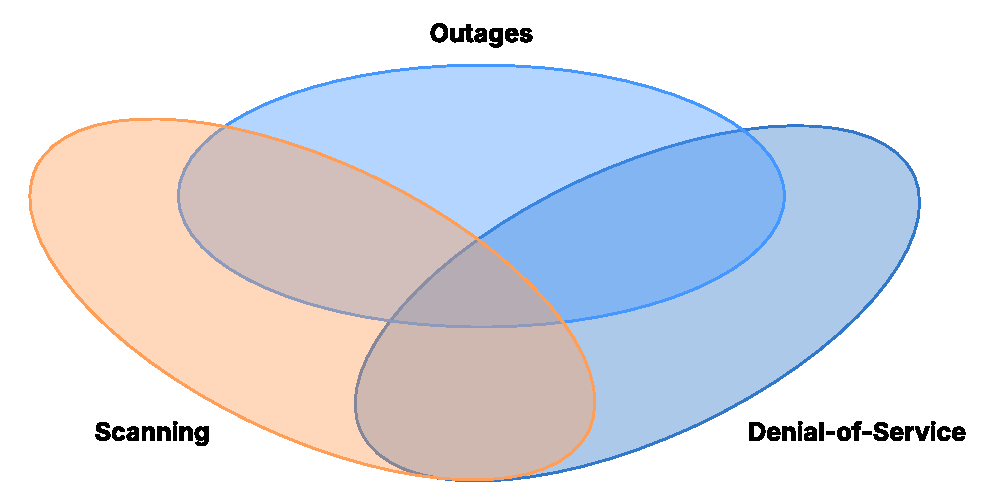
\includegraphics[]{figures/taxonomy.pdf}};
        \draw (-4, -4) node {Kallitsis et al.~\cite{2022kallitsis}};
    \end{tikzpicture}
    \caption{A taxonomy of our \maxnote{number} surveyed works and their methodologies categorized under the broad type of darknet activity they target and specific event definitions.}
    \label{fig:taxonomy}
\end{figure}

\subsection{Scan Detection}

A portion of darknet traffic mixtures results from scans that probe the space of Internet addresses, oftentimes targeting application-layer ports.
Detection of these scans involves identifying their sources and targets through analysis of behavioral patterns, thereby enabling further inference and/or classification of their intent.
This section provides a survey of the methodologies proposed for detecting scanning activities in darknet traffic. 

\noindent{\textbf{Sender Classification}}
Gioacchini et al.~\cite{2021gioacchini,2023gioacchini} propose a domain-specific adaptation of Word2Vec to embed senders based on their order of arrival from packet sequences \maxnote{defined over variations of port combinations}.
Kallitsis et al.~\cite{2022kallitsis} include a more comprehensive set of features to train autoencoders and subsequently cluster sender embeddings of a lower-dimensional space. 
Nishikaze et al.~\cite{2015nishikaze} cluster feature vectors that represent source /16 subnets and 27 selected features.
Zakroum et al.~\cite{2023zakroum} 

\vspace{0.25em}
\noindent{\textbf{}}
Han et al.~\cite{@@}, Kanehara et al.~\cite{@@}, and Kartsioukas et al.~\cite{@@} employ classic dimensionality reduction techniques, specifically on time-series representations of darknet traffic, alongside ad-hoc thresholding techniques to identify timeframes containing sources of coordinated scanning or targeted services by their ports.
These techniques include algorithms such as Non-negative matrix factorization (NMF)~\cite{@@}, Non-negative tucker-decomposition (NTD)~\cite{@@}, and Kartsioukas et al.~\cite{@@}, each of which reduce the space of potential source and destination tuples by filtering for those whose time series possess high reconstruction errors. 
Graphical LASSO~\cite{@@} instead focuses solely on sources by identifying non-trivial correlations in TCP-SYN packet volumes sent by source /16 subnetworks.

Another group of methods employ graph-mining techniques to model scanning behavior.
Evrard et al.~\cite{@@} and Lagraa et al.~\cite{@@} represent TCP scan traffic as unipartite graphs, where nodes represent ports and edges represent consecutive port scans, respectively on a global- and individual sender IP-basis. 
To extract similarly probed ports, Evrard et al.~\cite{@@} threshold a shortest-path similarity metric while Lagraa et al.~\cite{@@} instead threshold node centrality measures, such as degree centrality and betweenness measure, applied to a unified scan-graph.
In follow-up work, Lagraa et al.~\cite{@@} provide an additional graph definition aimed to detect horizontal scanners by redefining nodes as darknet destination addresses probed on the same port and employ an alternative clustering metric that measures graph modularity.
Soro et al.~\cite{@@} define weighted bipartite graphs that link source Autonomous Systems (ASes) to destination ports based on the number of packets in TCP scan traffic that ASes send and extract ASes that target similar sets of ports using the Greedy Modularity Algorithm.


\subsection{Backscatter Detection}
Several of the previously mentioned methodologies in Section~\ref{@@} detect both scans and backscatter since reflected response traffic generated by spoofed DoS attacks can resemble scanning behavior, e.g., a DoS victim's response to spoofed traffic compared to high-volume horizontal scans.
While distinguishing backscatter from scans in stateful protocol traffic such as TCP, e.g., by inspecting untampered TCP flags, for stateless protocols such as ICMP and UDP it is less so. 
\maxnote{enumerate works here}

\subsection{Outage Detection}
In contrast to scanning and backscatter detection, outage detection methodologies aim to identify the absence of expected traffic.
These methodologies frame detection in terms of traffic sources defined at varying spatial grains (e.g., per-subnet, per-AS, or per-country) which may depend on darknet-exogenous data for geolocation or AS-organization lookups.

Our survey identifies two works that propose complete outage detection methodologies.
Guillot et al. propose Chocolatine~\cite{2019guillot} which forecasts the expected number of unique senders aggregated at per-AS and per-country granularities by training a Seasonal Autoregressive Integrated Moving Average (SARIMA) model over historical sender counts of unfiltered, protocol-agnostic traffic inputs; 
sender counts beyond specified 5-minute prediction thresholds are flagged as potential outages.
Enyanet et al. propose Durbin~\cite{2024enyanet} which leverages a Bayesian approach for inferring outages down to a coarser spatial grain of a /24 subnetwork in comparison to Chocolatine. Furthermore, Durbin optimizes parameters per-subnet and and claims to more flexibly exploit space-time precision trade-offs by doing so. 

\begin{table}[t]
    \small
    \caption{Characteristics of event detection frameworks proposed in our surveyed literature (excluding algorithms).}
    \label{tab:frameworks-noalgos}
    \begin{tabular}{llllc}
        \toprule
        \multicolumn{1}{c}{Work} & \multicolumn{4}{c}{Framework} \\
        \midrule
        & \rot{45}{i. Activity} & \rot{45}{ii. Technique(s)} & \rot{45}{\begin{tabular}[c]{@{}l@{}}iv. Traffic\\ Rep.\end{tabular}} & \rot{45}{\begin{tabular}[c]{@{}l@{}}v. Output\\ Attributes\end{tabular}} \\
        \midrule
        Evrard et al.~\cite{2019evrard} & \markX & \markB & \markD & Dst. Port \\
        Lagraa et al.~\cite{2017lagraa,2019lagraa} & \markX & \markB & \markD & Dst. Port \\
        Kallitsis et al.~\cite{2022kallitsis} & \markX\markY & \markI\markA\markB & \markE & Src. IP \\
        Iglesias et al.~\cite{2019iglesias} & \markX\markY & \markB\markH & \markE & Src. IP \\
        Nishikaze et al.~\cite{2015nishikaze} & \markX & \markB & \markE & Src. /16 \\
        Soro et al.~\cite{2020soro} & \markX & \markB & \markF & Src. AS \\
        Gioacchini et al.~\cite{2021gioacchini,2023gioacchini} & \markX & \markA\markB & \markF & Src. IP \\
        Han et al.~\cite{2021han,2022han} & \markX & \markA & \markG & Src. /16, Dst. Port \\
        Han et al.~\cite{2020han,2022han} & \markX\markEtc & \markA & \markG & Src. /16 \\
        Kanehara et al.~\cite{2019kanehara,2022han} & \markX & \markA\markH & \markG & Src. /16, Dst. Port \\
        Kartsioukas et al.~\cite{2023kartsioukas} & \markX & \markA\markH & \markG & \textit{TODO} \\
        Ban et al.~\cite{2016ban} & \markX & \markA & \markF\markG & Dst. Port \\ 
        Torabi et al.~\cite{2020torabi,2018torabi} & \markX & \markJ & \markD,\markE & \textit{TODO} \\
        Tanaka et al.~\cite{2023tanaka,2021tanaka} & \markX & \textit{TODO} & Source & \textit{TODO} \\
        Niranjana et al.~\cite{2019niranjana} & \markX & \markA\markB & Source & \textit{TODO} \\
        Cabana et al.~\cite{2019cabana} & \markX & \markB\markH & \markD\markE & \textit{TODO} \\
        Shaikh et al.~\cite{2018shaikh} & \markX\markY\markZ\markEtc & \textit{TODO} & \markE & \textit{TODO} \\  
        Zakroum et al.~\cite{2022zakroum,2018zakroum} & \markX & \markC\markB & \markG & Dst. Port \\
        Zakroum et al.~\cite{2023zakroum} & \markX & \markC\markB & \markG & Dst. Port \\
        Guillot et al.~\cite{2019guillot} & \markZ& \markC\markB & \markG & Dst. Port \\
        Enyanet et al.~\cite{2024enyanet} & \markZ & \markC\markB & \markG & Dst. Port \\
        Zakroum et al.~\cite{2023zakroum} & \markX & \markC\markB & \markG & Dst. Port \\
        Guillot et al.~\cite{2019guillot} & \markZ& \markC\markB & \markG & Dst. Port \\
        Enyanet et al.~\cite{2024enyanet} & \markZ & \markC\markB & \markG & Dst. Port \\
        \bottomrule
    \end{tabular}

    \vspace{2pt}
    \parbox{\linewidth}{\raggedright
        \textit{Activities:} \markX~Scanning, \markY~DDoS, \markZ~Outage, \markEtc~Misconfiguration.\\
        \textit{Techniques:} \markA~Dimensionality Reduction, \markB~Clustering, \markC~Forecasting, \markH~Thresholding, \markI~Representation Learning, \markJ~Frequent Pattern Mining, \markH~Fingerprinting.\\
        \textit{Traffic representation:} \markD~Graph, \markE~Feature Vector, \markF~Sequences, \markG~Time Series.
    }
\end{table}



\label{sec:evaluations}
\section{Empirical Assessments of Detection Methodologies}

To demonstrate the utility of their detection methodologies, prior works conduct assessments using real-world darknet traffic datasets.
These assessments and their results provide evidence of a method's performance under realistic settings and offer empirical insights into its detection capabilities and general scalability.
In this section, we characterize prior works along the lines of credibility and reproducibility of their assessments by reviewing:
(i) characteristics of the darknet traffic datasets they use; and
(ii) their approach to validating detection outputs of their methodology.
Furthermore, we consider implementation details of detection methodologies since the reproducibility of assessments and results are closely tied to the availability of method source code and specifications of chosen computational environments.

\vspace{0.25em}
\noindent{\textbf{Characteristics of darknet traffic datasets.}}
For the datasets used in prior works, we consider several characteristics relevant to interpreting method assessment results:
the timeframe over which traffic was collected, the specific darknet that received this traffic, the size of the darknet's address space, and its traffic volume measured in units of packets and bytes.

\vspace{0.25em}
\noindent{\textbf{Validation of detection results.}}
We consider the soundness of method assessments by examining how prior works validate their method's detection outputs in the absence of well-defined ground truth; we identify 3 common approaches.
In the first approach, authors~\cite{@@} manually inspect detection outputs and interpret their meaning. This non-exhaustive approach to validation serves to illustrate method capabilities in an exploratory manner.
The second approach extends this process by cross-referencing detection outputs with external datasources, e.g., crowdsourced reports of scanners such as AbuseIPDB~\cite{@@}, \maxnote{enumerate}. Compared to the previous approach, confirmation provided by an additional source can improve confidence in result interpretations.
The third and most formal approach involves constructing labeled datasets prior to assessment and computing accuracy metrics, e.g., conventional information retrieval metrics such as precision, recall, or F1-score, from subsequently obtained outputs combined with labeled samples. While this approach is the most reproducible, sound comparison of validation results depends on objective definitions for labels.

% \begin{enumerate}
%     \item Some authors run their method, grab outputs, manually inspect and interpret the results.
%     \item Other authors first label their data, run their method, grab outputs, compute accuracy metrics using pre-labeled data.
%     \item Other authors run their method, grab outputs, join outputs against an external data source, and then interpret
% \end{enumerate}

\vspace{0.25em}
\noindent{\textbf{Replicability of detection methodologies.}}
We assess the replicability of each detection methodology by considering whether authors publicly release the source code or software artifacts of their methodology and whether they provide specifications of the computational environment in which they execute their assessments. 
Both factors enable other reasearchers to reproduce reported results for the same dataset or to apply the methodology to new datasets under similar conditions. 
While our review does not consider the quality or maintainability of the software, we note that these factors also play a role in method replicability.

% \begin{enumerate}
%     \item Sound comparisons of different methods depend on replicable implementations, i.e., available source code, distributable software, details of computational environment
%     \item Without these, the next best thing well-documented descriptions detection methodology itself (though this is prone to implementation errors)
%     \item \textit{Describe findings}
% \end{enumerate}

\section{A Need for A Systemized Evaluation of Darknet Event Detection Methodologies}

\begin{enumerate}
    \item From the combined survey of methods and their assessments, we find: a diverse set of available approaches that have yet to be completely compared.
    \item In this section, we drill down into the findings that led to this conclusion and details of these gaps.
\end{enumerate}

\noindent{\textbf{Side-by-side methodology comparisons.}}
Fewer than half of our surveyed works directly compare detection methodologies via evaluations on the same dataset.

% Evaluations that directly compare detection methodologies on the same dataset yield the most definitive results of their relative capabilities.
% Fewer than half of surveyed works fit this criteria 
% Evaluation of detection methodologies by directly comparing their Direct comparisons of detection methodologies yield
% Evaluation of detection methodologies  yield definitive results.
% Slightly fewer than half of our surveyed works evaluate their proposed methodology against a baseline methodology using the same dataset.
% Of those, use of a dataset does not extend beyond an individual work, i.e., real-world traffic datasets are not widely shared for researchers to evaluate their methodologies.


\begin{enumerate}
    \item direct comparisons of detection methodologies by evaluating them on the same dataset is the ideal scenario
    \item Slightly fewer than half of surveyed works fit this criteria
	\item we can't reasonably compare frameworks by their performance on different datasets.
	\item Few works compare different frameworks on the same dataset
	\item What's the highest number of frameworks that use the same dataset?
\end{enumerate}

\noindent{\textbf{Limited replicability of detection methodologies.}} 
Less than a third of studies publish source code of their methodologies and of those that do, their releases are seldom packaged as reusable libraries, distributed through package managers, or maintained beyond initial publication. 
While the primary goal of these studies is to disseminate research ideas rather than deliver production-grade software, their codebases nonetheless lack interfaces and clear documentation needed for straightforward implementation and thereby discourages frictionless replication.
% Less than a third of the studies publish accompanying source code of their framework implementation and of those that do, 
% we find that their releases are seldom packaged as reusable libraries, distributed through package managers, or maintained beyond initial publication.
% This aligns with expectations as the primary goal is to disseminate research ideas rather than deliver production-grade software.
% Nonetheless, the condition of the codebases we find often lack interfaces and clear documentation needed for straightforward implementation.

Slightly more than half of the works do, however, provide specifications of the computing environment, \textit{e.g., processor capabilities and memory capacity}, used to run evaluations.
\maxnote{add to significance}

\noindent{\textbf{Non-overlapping datasets used for experimentation.}}
\begin{enumerate}
    \item little overlap in the datasets used to evaluate frameworks
    % \item evaluation of detection methodologies use darknet traffic sourced from a variety of telescopes over different timeframes
    \item traffic volumes differ by multiple orders of magnitude.
    \item different sources of traffic
    \item mostly non-overlapping timeframes
\end{enumerate}

\begin{table*}[h!]
    \small
    % \centering
    \setlength{\tabcolsep}{4pt}
    \caption{Details of empirical evaluation and traffic datasets found in our surveyed work. Appx. Table~\ref{@@} summarizes referenced telescopes.}
	% \caption{Implementation and evaluation details of our surveyed work. Darknet owner indicates which telescope provided each dataset. Traffic volume is split into packets and bytes.}
    \label{tab:eval}
    \begin{tabular}{@{}lccccccccc@{}}
        \toprule
        & \multicolumn{1}{c}{\textbf{Compari-}} 
        & \multicolumn{2}{c}{\bf Replicability} 
        & \multicolumn{1}{c}{\textbf{Telescope(s)}} 
        & \multicolumn{4}{c}{\bf Dataset Attributes} 
        & \multicolumn{1}{c}{\textbf{Annot-}} \\
        \cmidrule(lr){3-4} \cmidrule(lr){6-9}
        \textbf{Work} & \textbf{son} & \textbf{Code} & \textbf{Specs} &  & \textbf{Duration} & \textbf{Year} & \textbf{Packets} & \textbf{Bytes} & \textbf{ations} \\
        \midrule
        Evrard et al.~\cite{2019evrard}
        &  
        &  & 
        & T3, T6
        & 9m & 2015
        & ${\approx}8\times10^{8}$ & ---
        & Manual \\

        Lagraa et al.~\cite{2017lagraa,2019lagraa}
        &  
        &  & \cmark
        & T6
        & 2y & 2014
        & $2\times10^{9}$ & 500 GB
        & Manual \\

        Soro et al.~\cite{2020soro}
        &  
        &  & 
        & T4
        & 3w & 2019
        & --- & ---
        & Manual \\

        Nishikaze et al.~\cite{2015nishikaze}
        &  
        &  & 
        & T3
        & 28d & 2014
        & $3.03\times10^{8}$ & ---
        &  Manual \\

        Kallitsis et al.~\cite{2022kallitsis}
        & \cite{2021gioacchini}
        & \cmark & \cmark
        & T2
        & 28d & 2016
        & $49\times10^{9}$ & ---
        & Manual, Labeled \\

        Iglesias et al.~\cite{2019iglesias}
        &  
        &  & \cmark
        & T1
        & 1m & 2012
        & --- & 2.1 TB
        &  Manual \\

        Gioacchini et al.~\cite{2021gioacchini,2023gioacchini}
        & \cite{2020cohen}
        & \cmark & \cmark
        & T4
        & 30d & 2021
        & $6.3\times10^{7}$ & ---
        & Labeled \\

        Cohen et al.~\cite{2020cohen}
        & \cite{2016ban}
        &  & \cmark
        & Ad hoc ($\approx$/22)
        & 1y & 2019
        & --- & $3+\,\mathrm{TB}$
        & \wc{manual} \\

        Han et al.~\cite{2021han,2022han}
        & \cite{2020han,2006takeuchi,2019kanehara}
        & \cmark & 
        & T3
        & 1m & 2018
        & --- & ---
        & \wc{manual} \\

        Han et al.~\cite{2020han,2022han}
        & \cite{2006takeuchi}
        & \cmark & \cmark
        & T3
        & 1m & 2018
        & --- & ---
        & \wc{manual} \\

        Kanehara et al.~\cite{2019kanehara,2022han}
        & 
        &  & \cmark
        & T3
        & 6m & 2018
        & --- &
        & \wc{manual} \\

        Ban et al.~\cite{2017ban}
        & \cite{2012ban}
        &  & 
        & T3
        & --- & ---
        & --- & ---
        & Manual \\

        Ban et al.~\cite{2016ban}
        & 
        &  & 
        & T3
        & 1y & 2015
        & $3\times10^{7}$ & ---
        & Manual \\

        Bou-Harb et al.~\cite{2014bouharb}
        &  
        &  & 
        & T7
        & 1m & 2013
        & --- & ---
        &  \\

        Bou-Harb et al.~\cite{2019bouharb,2015bouharb}
        & ~\cite{2018bouharb}
        &  & \cmark
        & T1,T7
        & 1m,1m & 2016,2014
        & --- & 670GB, 240GB
        & Approach 2 \\

        Zakroum et al.~\cite{2022zakroum,2018zakroum}
        & ~\cite{2018zakroum}
        & & \cmark
        & T3, T6
        & 3.5y & 2017
        & --- & $1.5+\mathrm{TB}$
        &  Approach 2 \\

        Zakroum et al.~\cite{2023zakroum}
        & ~\cite{2023zakroum}
        & &
        & T3, T6
        & 4.5y & 2018
        & --- & ---
        & Approach 3 \\

        \midrule
        \textbf{Aggregate}
        & 7/16
        & 4/16 & 7/16
        & 8-24
        & 1w--3.5y & 2012--2021
        & --- & ---
        & --- \\
        \bottomrule
    \end{tabular}
\end{table*}

\label{sec:fw}
\section{Future Work}

\begin{enumerate}
    \item We discuss how to address the gaps we identified from our survey by providing ideas 
    \item We discuss how to address the gaps we identified from our survey by providing ideas 
    \item we need a systematic approach to do this, which depends on addressing the limitations mentioned in previous section.
    \item 
\end{enumerate}

\noindent{\textbf{Curated datasets.}}
\begin{enumerate}
    \item Sound comparisons between methods rely on shared datasets whose characteristics are well-documented.
    \item Traffic within these datasets that are associated with major events should be labeled.
    \item Label definitions can be flexible, but there needs to be agreement on their definitions.
    \item Examples include signatures of scanning tools, scanning organizations based on registered address ranges, or the outputs of previously assessed detection methodologies
    \item Sound comparisons between methods rely on shared datasets whose characteristics are well-documented.
    \item Traffic within these datasets that are associated with major events should be labeled.
    \item Label definitions can be flexible, but there needs to be agreement on their definitions.
    \item Examples include signatures of scanning tools, scanning organizations based on registered address ranges, or the outputs of previously assessed detection methodologies
\end{enumerate}

\noindent{\textbf{Systematic evaluation.}}

Although some individual works from our survey evaluate their methodologies with the same metrics, \textit{e.g.,} TP, FP, \dots, 
the

\begin{enumerate}
	\item Discuss need for standardized evaluation metrics
	\item Discuss need for experimental consistency
	\item These depend on reusability of framework implementations
\end{enumerate}

% \section{Acknowledgments}
% asadfadsf

\section{Appendices}

\begin{table}[httb]
	\small
	\caption{Summary of network telescopes.}\label{tab:telescopes}
	\begin{tabular}{cccc}
		\toprule
		Telescopes & Country & Size & Data availability\\
		\midrule
		\textbf{T1.} UCSD-NT~\cite{caida2025ucsdnt} & US & /9+/10 & Raw traces and flow data \\
		\textbf{T2.} Merit ORION~\cite{orion} & US & $\sim$7 $\times$/16s & Raw trace\\
		\textbf{T3.} NICTER~\cite{nicter2025nt} & JP &  /17, /18, 2$\times$/20 & TCP SYN only, anonymized flow data\\
		\textbf{T4.} Politecnico di Torino \cite{2020soro} & IT & 3 $\times$ /24 & Unknown\\
		\textbf{T5.} Darknet-BR \cite{CunhaCamargo2025darknetbr} & BR & /19 & Unknown\\
		\textbf{T6.} LHS Nancy~\cite{inria2025nt} & FR & /20 & Raw trace\\
		\textbf{T7.} Farsight~\cite{@@} & US & /13 & Private\\
		\bottomrule
	\end{tabular}
\end{table}

\begin{table}[]
    \small
    \caption{Algorithms used by each surveyed framework.}
    \label{tab:frameworks-algorithms}
    % Use p{<width>} to allow wrapping of long algorithm lists.
    \begin{tabular}{lp{0.62\linewidth}}
        \toprule
        \textbf{Work} & \textbf{Algorithm(s)} \\
        \midrule
        Evrard et al.~\cite{2019evrard}                        & Dijkstra's~\cite{1959dijkstra}; K-NN~\cite{1967cover,1989fix} \\
        Lagraa et al.~\cite{2017lagraa,2019lagraa}             & Louvain~\cite{2006newman,2008blondel} \\
        Kallitsis et al.~\cite{2022kallitsis}                  & Autoencoder Dimensionality Reduction~\cite{2006hinton}; K-Means~\cite{1967macqueen} \\
        Iglesias et al.~\cite{2019iglesias}                    & K-Medoids~\cite{2009park}; Fuzzy-Gustafson~\cite{1999krishnapuram}; MAD-Thresholding~\cite{2004liu} \\
        Nishikaze et al.~\cite{2015nishikaze}                  & Hierarchical Clustering~\cite{2012murtagh} \\
        Soro et al.~\cite{2020soro}                            & Louvain Algorithm~\cite{2006newman,2008blondel} \\
        Gioacchini et al.~\cite{2021gioacchini,2023gioacchini} & Word2Vec~\cite{2013mikolov}; K-Means~\cite{1967macqueen}; K-NN~\cite{1967cover,1989fix}; Louvain~\cite{2006newman,2008blondel} \\
        Han et al.~\cite{2021han,2022han}                      & NMF~\cite{2000lee} \\
        Han et al.~\cite{2020han,2022han}                      & GLASSO~\cite{2008friedman} \\
        Kanehara et al.~\cite{2019kanehara,2022han}            & LRA-NTD~\cite{2015zhou}; FTSD~\cite{2010caiafa}; Otsu-Thresholding~\cite{1979otsu} \\
        Kartsioukas et al.~\cite{2023kartsioukas}              & Incremental PCA~\cite{2012arora} \\
        Ban et al.~\cite{2016ban}                              & Frequent Pattern Mining~\cite{2000han,2007han}; Hierarchical Clustering~\cite{2012murtagh} \\
        Torabi et al.~\cite{2020torabi,2018torabi}             & Association Rule Mining~\cite{1993agrawal}; DBSCAN~\cite{1996ester} \\
        Tanaka et al.~\cite{2023tanaka,2021tanaka}             & \textit{TODO} \\
        Niranjana et al.~\cite{2019niranjana}                  & PCA~\cite{1901pearson,1993hotelling} \\
        Cabana et al.~\cite{2019cabana}                        & Conduction Detection Algorithm~\cite{2015lu}; Fastcluster~\cite{2013mullner} \\
        Shaikh et al.~\cite{2018shaikh}                        & AdaBoost~\cite{@@}; Gradient Boosting~\cite{@@}; Random Forest~\cite{@@} \\
        Zakroum et al.~\cite{2022zakroum,2018zakroum}          & Spectral Clustering~\cite{2001ng}; LSTM~\cite{1997hochreiter} \\
        \bottomrule
    \end{tabular}
\end{table}


\begin{acks}
To Robert, for the bagels and explaining CMYK and color spaces.
\end{acks}

\bibliographystyle{plain}
\bibliography{bib/refs.bib}

\appendix
\section{Research Methods}

\subsection{Part One}

Lorem ipsum dolor sit amet, consectetur adipiscing elit. Morbi
malesuada, quam in pulvinar varius, metus nunc fermentum urna, id
sollicitudin purus odio sit amet enim. Aliquam ullamcorper eu ipsum
vel mollis. Curabitur quis dictum nisl. Phasellus vel semper risus, et
lacinia dolor. Integer ultricies commodo sem nec semper.

\end{document}
\endinput